\chapter{Software}

Wireless sensor networks must be reliable. If a network mote fails, motes connected to the failed device must find another path to reliably transmit data to a base station. At the same time, wireless sensor networks must be scalable. A sensor network should be able to handle the addition of any number of new devices. The software described in this thesis supports reliable and scalable wireless sensor networks. We rely on the following terms throughout the exposition :
\begin{enumerate}
\item \textit{base station} : A \textit{base station} is a field deployed server machine which receives, processes, analyzes, and stores the data received from the motes.
\item \textit{level} : The \textit{level} of a mote is the distance (in hops) of the mote from a \textit{base station}.
\item \textit{parent} : The \textit{parent} of a mote \textit{A} is the mote to which \textit{A} is connected. Its \textit{level} is one \textit{level} less than that of \textit{A}.
\item \textit{child} : A \textit{child} of a mote \textit{B} is the mote connected to \textit{B}, with \textit{B} serving as its \textit{parent}. Its \textit{level} is one \textit{level} more than that of \textit{A}.
\end{enumerate}

\section{Mote States}
In our system, every mote in the network is in one of the following four states:
\begin{enumerate}
\item \textbf{\textit{root}}\\The \textbf{\textit{root}} state indicates that the current mote is directly connected to a base station. All the messages received by this mote are forwarded directly to the base station. All other motes in the network are synchronized with the local clock of this mote. The \textbf{\textit{root}} mote periodically transmits a \textbf{\textit{sync}} signal to its children, and in response, the children transmit data to the \textbf{\textit{root}}.
\item \textbf{\textit{idle}}: \\The \textbf{\textit{idle}} state indicates that the mote is not connected to any other motes; it is searching for a \textit{parent}. All the motes except the \textbf{\textit{root}} mote are in the \textbf{\textit{idle}} state at boot. \textbf{\textit{idle}} motes periodically send a beacon and try to connect to a responding mote.
\item \textbf{\textit{leaf}}: \\The \textbf{\textit{leaf}} state indicates that the mote is now connected to a \textit{parent}. It also indicates that the mote can transmit its data to the base station through its \textit{parent}. The mote enters the \textbf{\textit{leaf}} state from the \textbf{\textit{idle}} state.
\item \textbf{\textit{node}}: \\The \textbf{\textit{node}} state indicates that the mote is connected to a \textit{parent} and other motes are connected to it as children. In this state, the mote will periodically send a \textbf{\textit{sync}} signal to its children and receive sensor data in response.  Each \textbf{\textit{node}} will transmit the received data along with its own data to its \textit{parent}, which will in turn continue to relay data until it reaches the base station.
\end{enumerate}

\section{Software Services}
The software described in this thesis provides four major functions : time synchronization, transmission slot management, parent search, and data transmission. We describe the design of these facilities in the following subsections.
%Time synchronization is an important factor in wireless sensor networks. In typical applications, motes do important work only for a short duration and spend most of their time doing nothing. Further, wireless sensor networks are prone to channel congestion, leading to packet loss and excessive power consumption. To reduce channel congestion, we use synchronized transmission slots.
%\item Deepsleep or sleep when generating delay

\subsection{Time Synchronization}
Time synchronization is an important factor in wireless sensor networks. In typical applications, motes do important work only for short periods; most of the time they are idle. The majority of the total power consumption stems from the radio. To conserve power, the radio must be turned off and switched on only when required. If a transmitting mote and the corresponding receiver are not synchronized, the data will be lost. This problem is exacerbated if the network is multi-hop. To achieve reliable multi-hop communication, every mote must be time synchronized and must know when to transmit and receive data so there is no packet loss.

To achieve time synchronization, every mote maintains a local clock. We use the internal Timer2 of the ATMEGA168 microcontroller. Timer2 is programmed to generate an interrupt every millisecond. The interrupt handler increments the count of the local clock by one, creating a millisecond timer. Timer2 computes this time based on the cycles generated by the internal resistor-capacitor (RC) oscillator. Unfortunately, in practical situations, the generated clock is not perfect; its accuracy depends on factors including temperature and humidity. Due to these dependencies, the error rate of the RC oscillator is quite high: $\pm$ 10\% \cite{bib_atmega}. To overcome this, motes are synchronized frequently.

Commonly used time synchronization protocols in wireless sensor networks include Flooding Time Synchronization Protocol (FTSP), Reference Broadcast Synchronization (RBS), and Timing-sync Protocol for Sensor Networks (TPSN).

A significant problem in using the FTSP, RBS, and TPSN time synchronization protocols is that each assumes the motes in the network will always be on. This thesis combines the best features of FTSP and TPSN to achieve time synchronization across the network. In this design, the network is hierarchical. Each parent in the routing tree transmits a synchronization (SYNC) packet only when checking whether its child has data to transmit. If data is transmitted every minute, the parent will send a SYNC packet every minute. As soon as a child receives a SYNC packet, it sets its clock based on the clock of its parent, and then transmits its data packet to its parent. Instead of concentrating on network-wide synchronization, this approach focuses on synchronization between parents and children, which indirectly synchronizes the whole network. This in turn eliminates the need for unnecessary broadcast packets, which saves power and reduces the likelihood of network congestion.

Another problem in implementing time synchronization is clock drift. We know that the error rate of the RC oscillator is $\pm$ 10\%, causing drift in the local clock of every mote. To minimize clock drift, each clock maintains a variable that contains the measured drift between it and its parent. The transmission interval between synchronization packets is the same throughout the network. Further, holding external factors constant, the drift in clock time between a pair of motes will always be the same between two consecutive synchronization packets. We calculate the clock drift by subtracting the value of the local clock of the child with the local clock of the parent. To minimize clock drift, each time a synchronization packet is received, the difference is added to the local clock of the parent and stored in the local clock of the child.
%If this difference is added to the local clock of the parent and stored in the local clock of the child each time a synchronization packet is received, the problem of clock drift can be minimized.

\subsection{Transmission Slots}\label{sec:trans_slots}
Wireless sensor networks are prone to channel congestion, leading to packet loss and excessive power consumption. To reduce channel congestion, this thesis makes use of synchronized transmission slots. Each parent assigns transmission slots to its children. A parent and child can communicate only during this time. The parent cannot assign the same transmission slot to multiple children.

The duration of a transmission slot is calculated based on the time required to transmit a packet with a maximum payload. Specifically, it is twenty times the time required to transmit a packet with a maximum payload. In the worst case, the transmitter can resend data nineteen times (assuming no delay), which in most cases is enough for the data to reach the receiver.

\begin{equation}
T_{ts} = 20*T_{mp}
\end{equation}
%where,\\
%$T_{ts}$ = time duration of a transmission slot\\
%$T_{mp}$ = time required to transmit a packet with maximum payload

\begin{tabular}{lllp{10cm}}
where, & • & • & • \\ 
• & $T_{ts}$ & = & Time duration of a transmission slot \\ 
• & $T_{mp}$ & = & Time required to transmit a packet with maximum payload \\ 
\end{tabular} 

\begin{equation}
T_{mp} = \frac{8*(maximum\ size\ of\ payload\ (in\ bytes)\ +\ packet\ overhead\ (in\ bytes))}{baudrate\ of\ radio\ (in\ bits\ per\ sec)}\ +\ backoff\ delay
\end{equation}
$T_{mp}$ = $\dfrac{8*(255\ +\ 10)}{57600}\ +\ 3*\dfrac{8*(255\ +\ 10)}{57600}$ = $147.24\ millisecond$\\
$T_{ts}$ = $20*147.24$ = $2944.8\ millisecond$ = $2.9448\ second$

%The time duration of the transmission slot also depends on the time required for a new mote to join the network. If the new mote broadcasts the connecting signal with period $t$, and $t$ is greater than half of $354.2$ millisecond then the time duration of the transmission slot is twice of $t$.

Transmission slots reduce the power consumption of each mote. A mote is powered up only during its assigned transmission slots (to communicate with its parent and children); otherwise, it is sleeping.

%\section{Deepsleep}The life of wireless sensor network depends on the power consumption of the motes. To increase the lifetime of sensor network, we must reduce the power consumption of the motes. This can be accomplished by switching off the components which are not in use.The mote must keep track of time in order to switch off the components without missing transmissions. We can keep track of time by using the local clock of the mote, but it will wake the mote every millisecond to increment the local time. To solve the problem of waking up mote every millisecond this thesis has a component called deepsleep. Deepsleep uses the internal Timer2 of ATMEGA168 for its operation. Instead of waking up mote every millisecond deepsleep waits for the maximum wait time. Then it wakes the mote and add that time to local clock. This process is repeated until the sleep time is not complete. If the sleep time is less than the maximum wait time of deepsleep, then the mote waits only until the sleep time.

\subsection{Parent Search}
This section discusses the steps taken by a mote to join the network.
\begin{figure}[htbp]
\centering
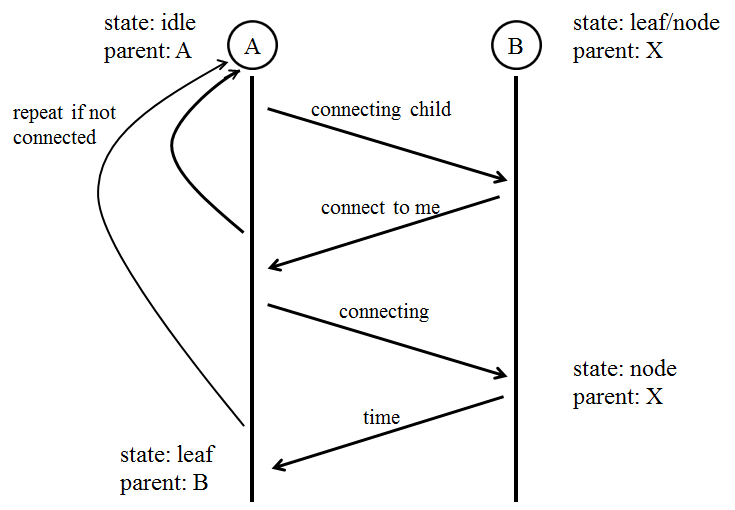
\includegraphics[width=\columnwidth]{algorithm1.png}
\caption{Finding a Parent Mote in the Network}
\label{img_algorithm1}
\end{figure}

As shown in Figure \ref{img_algorithm1}, mote A is in the \textit{\textbf{idle}} state, searching for a parent. Mote B is in the \textit{\textbf{leaf}} or the \textit{\textbf{node}} state. Mote B is connected to the tree, and mote X is the parent of mote B. In the \textit{\textbf{idle}} state, mote A broadcasts CONNECTING CHILD with period $t$. If there is another mote in the network which is time synchronized and has a transmission slot available, say B, it receives this message and transmits the CONNECT TO ME signal to mote A after some random time $\bar{t}$, where $(\bar{t} << t)$. When mote A receives the CONNECT TO ME signal from mote B, it transmits the CONNECTING signal to mote B. As soon as mote B receives the CONNECTING signal, it searches for an available transmission slot and assigns that transmission slot to mote A. It sends the TIME signal and sets its state to the \textit{\textbf{node}} state. Mote B then sets mote A as its child. As soon as mote A receives the TIME signal, it sets its local time to that of mote B, sets its state to \textit{\textbf{leaf}}, and sets mote B as its parent.

\subsection{Data Transmission}
\begin{figure}[htbp]
\centering
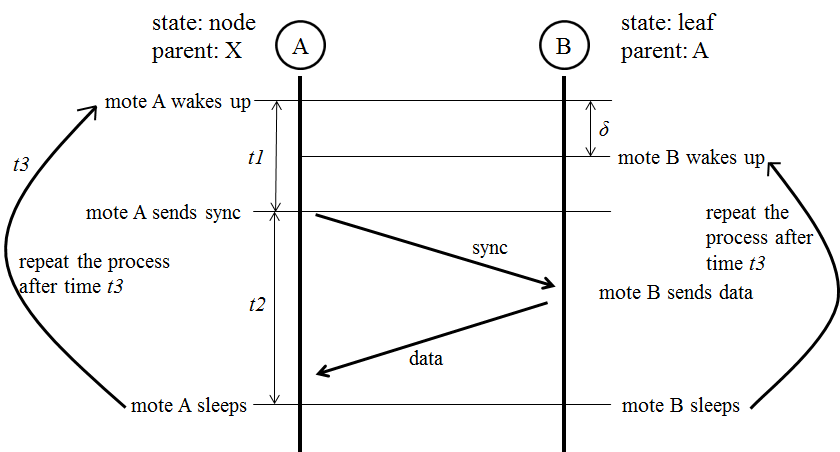
\includegraphics[width=\columnwidth]{algorithm2.png}
\caption{Sending the Sync Signal and Receiving Data}
\label{img_algorithm2}
\end{figure}

The main task of any network is to enable communication. This section discusses how data transmission takes place in our sensing system.

In Figure \ref{img_algorithm2}, mote A is in the \textit{\textbf{node}} state, and mote B is in the \textit{\textbf{leaf}} state. Mote A is the parent of mote B. When mote A wakes, it transmits the SYNC signal to its child, say B, after a delay of time $t1$. Mote A waits for time $t1$ to make sure that mote B is on; there might be a delay in waking mote B due to clock drift. Next, mote A waits up to the duration of a transmission slot, say $t2$, to receive DATA from its child. If mote A has multiple children, the process of sending the SYNC signal is repeated multiple times. Finally, after receiving DATA from all its children, mote A sleeps for time $t3$, and the above process is repeated.

As shown in Figure \ref{img_algorithm2}, mote B wakes up at time $\delta$. As soon as mote B receives the SYNC signal from its parent, it waits for a random amount of time before transmitting to avoid a collision. It then transmits the DATA to its parent mote. Next, mote B sleeps for time $t3$. This process is then repeated.

\subsubsection{Heartbeat Mechanism}
Data transmissions also help to detect motes which have failed. Data packets serve as the heartbeat of the network. When a mote fails, other motes detect this failure to maintain the overall health of the network. Network healing is one of the most important factors that makes data transmission in a network reliable.

When a parent fails, a child mote must detect it. To detect the death of a parent, every child maintains a variable, $parent\_life$. Whenever a child receives a SYNC signal from its parent, it sets $parent\_life$ to a predefined value. When a child wakes up from sleep, it decrements $parent\_life$ by one. If $parent\_life$ becomes zero, the child declares its parent dead and transmits the PARENT DYING signal to its children. Next, the child begins searching for another parent.

When a child mote fails, the parent mote must detect it. To detect the death of a child, say, $\textit{child}_{i}$, every parent maintains a variable, $child\_life_{i}$, specific to that child. When $\textit{child}_{i}$ gets connected to a parent, the parent sets $child\_life_{i}$ to a predefined value. Whenever a parent transmits a SYNC signal to $\textit{child}_{i},$ it decrements $child\_life_{i}$ by one. If the parent receives DATA from $\textit{child}_{i}$, it again sets $child\_life_{i}$ to its predefined value. If $child\_life_{i}$ becomes zero, the parent declares $\textit{child}_{i}$ dead. It then frees the transmission slot of that child and makes it available for a new child.

%\subsection{Working}
%This section describes the working of our software.

%In this software the parent periodically transmits synchronization packet to its children. The parent then waits for a specific time for receiving data from its children. The parent then sleeps for a predefined time to save power. When a new mote wants to join a network it begins searching for parent.

\section{Packet Formats}
This section discusses the packet formats used by the software for communication. The packets used for communication include (\romannumeral1) CONNECTING CHILD, (\romannumeral2) CONNECT TO ME, (\romannumeral3) CONNECTING, (\romannumeral4) TIME, (\romannumeral5) SYNC, (\romannumeral6) DATA, and (\romannumeral7) PARENT DYING. Each of these packets uses the packet format shown in Table \ref{tab:packet_format}.

\begin{table}[htbp]
\begin{center}
\begin{tabular}{|c|c|c|c|c|c|}
\hline 
\textit{\textbf{destination address}} & \textit{\textbf{source address}} & \textit{\textbf{flag}} & \textit{\textbf{length}} & \textit{\textbf{payload}} & \textit{\textbf{crc}} \\ 
(1 byte) & (1 byte) & (1 byte) & (1 byte) & (255 bytes) & (1 byte) \\ 
\hline 
\end{tabular}
\begin{tabular}{|l|l|}
\hline 
\textit{\textbf{destination address}} & The address of the destination mote \\ 
\hline 
\textit{\textbf{source address}} & The address of the transmitting mote \\ 
\hline 
\textit{\textbf{flag}} & Indicates whether the current packet is a data packet or an\\
 &  acknowledgment \\ 
\hline 
\textit{\textbf{length}} & Contains the size of the payload \\ 
\hline 
\textit{\textbf{payload}} & Contains the message \\ 
\hline 
\textit{\textbf{crc}} & Contains the cyclic redundancy check (CRC-8) computed over\\
 & the payload \\ 
\hline 
\end{tabular}
\caption{Packet Format}
\label{tab:packet_format}
\end{center}
\end{table}

\subsection{Payload Format}
This section summarizes the payload formats of the packets used by the software.
\begin{enumerate}
\item CONNECTING CHILD: The \textit{\textbf{payload}} format of a CONNECTING CHILD message is as follows:\\
\begin{tabular}{|c|}
\hline 
\textit{\textbf{CONNECTING CHILD}} (1 byte) \\ 
\hline 
\end{tabular}

Here, the \textit{\textbf{CONNECTING CHILD}} field contains the CONNECTING CHILD token.
\item CONNECT TO ME: The \textit{\textbf{payload}} format of a CONNECT TO ME message is as follows:\\
\begin{tabular}{|c|c|}
\hline 
\textit{\textbf{CONNECT TO ME}} (1 byte) & \textit{\textbf{level}} (4 bytes) \\ 
\hline 
\end{tabular}

Here, the \textit{\textbf{CONNECT TO ME}} field contains the CONNECT TO ME token. The \textit{\textbf{level}} field contains the \textit{level} of the transmitting mote.

\item CONNECTING: The \textit{\textbf{payload}} format of a CONNECTING message is as follows:\\
\begin{tabular}{|c|}
\hline 
\textit{\textbf{CONNECTING}} (1 byte) \\ 
\hline 
\end{tabular}

Here, the \textit{\textbf{CONNECTING}} field contains the CONNECTING token.
\item TIME: The \textit{\textbf{payload}} format of a TIME message is as follows:\\
\begin{tabular}{|c|c|}
\hline 
\textit{\textbf{TIME}} (1 byte) & \textit{\textbf{transmission slot}} (4 bytes) \\ 
\hline 
\end{tabular} 

Here, the \textit{\textbf{TIME}} field contains the TIME token. The \textit{\textbf{transmission slot}} field contains the time slot of the receiving mote.
\item SYNC: The \textit{\textbf{payload}} format of a SYNC message is as follows:\\
\begin{tabular}{|c|c|}
\hline 
\textit{\textbf{SYNC}} (1 byte) & \textit{\textbf{local time}} (4 bytes) \\ 
\hline 
\end{tabular} 

Here, the \textit{\textbf{SYNC}} field contains the SYNC token. The \textit{\textbf{local time}} field contains the local time of the transmitting mote.
\item DATA: The \textit{\textbf{payload}} format of a DATA message is as follows:

\begin{tabular}{|c|c|c|c|}
\hline 
\textit{\textbf{DATA}} (1 byte) & \textit{\textbf{source address}} (1 byte) & \textit{\textbf{parent address}} (1 byte) & \textit{\textbf{message number}} (4 bytes) \\ 
\hline 
\end{tabular} 

Here, the \textit{\textbf{DATA}} field contains the DATA token. The \textit{\textbf{source address}} field contains the address of the transmitting mote. The \textit{\textbf{parent address}} field contains the address of the transmitting mote's parent. The \textit{\textbf{message number}} field contains the message number of the packet being transmitted by the transmitting mote. In real applications, this data packet would be extended to include the sensor's control data.
\item PARENT DYING: The \textit{\textbf{payload}} format of a PARENT DYING message is as follows:\\
\begin{tabular}{|c|}
\hline 
\textit{\textbf{PARENT DYING}} (1 byte) \\ 
\hline 
\end{tabular} 

Here, the \textit{\textbf{PARENT DYING}} field contains the PARENT DYING token.
\end{enumerate}

%The summary of the process of the software is as follows:
%\begin{enumerate}
%\item If a new mote wants to join a network it searches for a \textit{parent}.
%\item Data communication and time synchronization takes place between a \textit{parent} and \textit{child}.
%\item The motes then sleep for some specific time to save power.
%\item The above steps are then repeated.
%\end{enumerate}



\newpage


%\section{Program}

%This program performs following set of operations:
%\begin{itemize}
%\item Operation 1:\\ Whenever a mote is in Idle state, it broadcasts \textit{CONNECTING CHILD} signal and waits for some fixed amount of time T. If it doesn't hear anything from other motes then it transmits the signal again and this is repeated till it is not connected to any mote. After connecting it changes its status from idle to Leaf. At this point the mote starts a counter which is twice the period of the data transmission. If it doesn't receive \textit{SYNC} signal between this time then it resets itself and change its state from Leaf to idle.

%\item Operation 2:\\ Whenever a mote which is in state of Node or Leaf, is time synchronized, and has time slots available for new child listens to the \textit{CONNECTING CHILD} signal, It randomly waits for some amount of time between 0 to t1 to avoid collision and transmits the \textit{CONNECT ME} signal with its level embedded inside the packet to the mote from which it received the \textit{CONNECTING CHILD} signal.

%\item Operation 3:\\ Whenever the mote who broadcast the \textit{CONNECTING CHILD} signal and is not connected to any other mote in the mean while receives the \textit{CONNECT ME} signal it extracts the level information of the sending mote from the packet and compares it with its level information and if that value is less than its current level value, then it transmits the \textit{CONNECTING} signal to the mote from which it received the \textit{CONNECT ME} signal.

%\item Operation 4:\\ Whenever the mote who transmitted the \textit{CONNECT ME} signal and if it still has empty time slots receives the \textit{CONNECTING} signal from the mote to which it transmitted the \textit{CONNECT ME} signal, it finds the time slot which is empty and transmits the \textit{TIME} signal along with the time slot embedded in the packet to the mote from which it received the \textit{CONNECTING} signal. After it receives the confirmation message from that mote in the form of acknowledgment it sets the child address for that time slot to the address of that mote and sets its life to some specific value. It then decrements the amount of time slots available by one and sets its status as Node, except if it is Root.

%\item Operation 5:\\ Whenever the mote who transmitted the \textit{CONNECTING} signal and if it still not connected to any mote receives the \textit{TIME} signal from the mote to which it transmitted the \textit{CONNECTING} signal, it extracts the time slot from the packet and sets its time slot to that value. It also sets the address of the mote from which it received the \textit{TIME} signal as its parent address and sets the life of its parent to some specific value. It also sets its level to level+1 of the transmitting mote and changes its state from idle to Leaf.

%\item Operation 6:\\ Whenever any mote receives the \textit{SYNC} signal from its parent mote, it calculates the difference between the time received and its local time and if difference is positive it adds that difference to a variable which maintains this difference. If this difference is above specific value then the difference variable is set to zero. It then sets its local time by adding the time received and the variable which stores the difference in time. The mote then sets the life of its parent to some specific value. It randomly waits for some amount of time between 0 to t2 to avoid collision and transmits the \textit{DATA} signal with the data embedded inside the packet to its parent and waits for the acknowledgement. If it receives the acknowledgment it deletes the data else it transmit it again next time till the time it is not received.

%\item Operation 7:\\ Whenever the current mote receives the \textit{DATA} signal from its child it sets the life of that child mote to some specific value. It the current mote has the status of Root then it transfers this received data to the base station else if the current mote has the status of Node then it saves this data in internal buffer and transmits it later to its parent.

%\item Operation 8:\\ Whenever the current mote receives the \textit{PARENT DYING} signal from its parent, it sets the life of the  parent to zero so that it can propagate the death of the parent whenever it communicate with its child.
%\end{itemize}
